\section{Graph Theory} \label{sec:graph-theory}
Many problems in Machine Learning (ML) do not involve classification or prediction of single data points in isolation, but of sets of entities that may present a more, or less, complex relation with each other. 
Most real-world phenomena fit into the latter framework.
Graphs are one of the most powerful tools for the modelling of this class of problems, as their structure naturally captures the wide variety of relations that may exist between entities.
These range from the atomic structure of a molecule to a social network of friends.  
In both these examples graphs help in reasoning, visualising and making inferences and predictions.

\subsection{Graphs} \label{subsec:graphs}
\begin{definition}[Directed Graph]
	A directed graph is a tuple 
	\begin{equation*}
		\mathcal{G} = (\mathcal{V}, \mathcal{E}) \,,
	\end{equation*}
with $\mathcal{V} = \{ v_1 \ldots v_n \}$ the set of vertices/nodes and $\mathcal{E}\subseteq \mathcal{V} \times \mathcal{V}$ the set of edges.
\end{definition}
We will not be needing the subclass known as \textit{undirected graphs} that are characterised by $\mathcal{E}$ being a \textit{set} of unordered pairs, that is of sets of the form $\{x,y\}$, with $x,y \in \mathcal{V}$.

The class of graphs presently of interest are those where there can be at most a single directed edge between any pair of nodes in $\mathcal{V}$; that is, we are not considering \textit{multigraphs}.
We are also interested in enforcing that there be no \textit{cycles} in the graph so there can be no subset of edges in $\mathcal{E}$ that when followed from vertex $v_i$ eventually ends up in $v_i$ again.
A cycle is a \textit{walk} - a sequence of edges which joins a sequence of vertices - of nodes of the form $v_i, v_j, \cdots, v_i$ i.e., a walk where only the first and last vertex are repeated.
Thus we have also automatically excluded the special case of cycle called \textit{self-loop}: an edge from a node to itself. 
The resulting graph possessing only directed edges and no cycles is commonly called a \textit{directed acyclic graph}, or DAG for short.  
\begin{definition}[Directed Acyclic Graph] \label{def:dag}
	A directed acyclic graph is a graph where every edge is directed and there are no cycles.
\end{definition}

In a DAG we may qualify nodes based on their \enquote{relationship status}:
\begin{description}
	\item[children] The children of node $u$ are all nodes $k$ for which there is a \textit{directed edge} from $u$ to $k$
	\item[parents] The parents of node $u$ are all nodes $k$ for which there is a \textit{directed edge} from $k$ to $u$
	\item[descendants] The descendants of node $u$ are all nodes $k$ for which there is a \textit{directed path} i.e., a walk where all vertices are distinct, from $u$ to $k$
	\item[ancestors] The ancestors of $u$ are all nodes for which there is a directed path from $k$ to $u$
\end{description}

An example of a DAG, containing five nodes, is shown in Figure \ref{fig:bn-example-dag}.

\begin{figure}[htbp]
\centerline{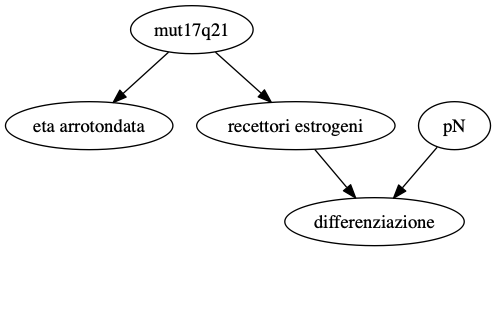
\includegraphics[width=0.5\textwidth]{mathematical-background/images/bn-example-structure}}
\caption{Example DAG representing a subset of the data set used in this thesis}
\label{fig:bn-example-dag}
\end{figure}

Polytrees and trees will also be defined because these are a fundamental concept for the work carried out in this thesis.
\begin{definition}[Tree] \label{def:tree}
	A tree is an undirected graph where there is one and only one walk between every node.	
\end{definition}
\begin{definition}[Polytree] \label{def:polytree}
	A polytree is a DAG whose underlying undirected graph is a tree.
	That is, if the directionality of edges is removed from the DAG, the resulting object is a tree. 
\end{definition}

\subsection{D-separation} \label{subsec:d-separation}
\textit{Dependence-separation} or \textit{d-separation}, as the name entails, is a concept relating to the conditional dependence between variables and was first presented by \citet{Pearl1988}.
We define the notation $u \rightarrow v$ to signify that there is a \textit{trail} between $u$ and $v$ in the graph, with a trail $(u, \ldots ,v)$ being a walk where all edges are distinct.

$u$ and $v$ and a node $z \in Z$ may be arranged in the graph in one of the following four configurations, called \textit{v-structures} in this context:
\begin{itemize}
  \item \textit{chain}: $u \rightarrow z \rightarrow v$
  \item \textit{chain}: $u \leftarrow z \leftarrow v$
  \item \textit{fork}: $u \leftarrow z \rightarrow v$
  \item \textit{collider}: $u \rightarrow z \leftarrow v$
\end{itemize}

These v-structures may be \textit{closed} by the set $Z$, this happens when:
\begin{itemize}
  \item \textit{chain}: $u \rightarrow z \rightarrow v$ and $z \in Z$
  \item \textit{chain}: $u \leftarrow z \leftarrow v$ and $z \in Z$
  \item \textit{fork}: $u \leftarrow z \rightarrow v$ and $z \in Z$
  \item \textit{collider}: $u \rightarrow z \leftarrow v$ and $z \notin Z$ and no descendant $z'$ of $z$ i.e., $z'$ such that $z \rightarrow z'$ exists, is also in the set $Z$
\end{itemize}

We say that $u$ and $v$ are \textit{d-separated} by $Z$ if every v-structure they appear in, is closed by $Z$.
Conversely, if there is at least one \textit{open} v-structure $u$ and $v$ are \textit{d-connected}.

If $u$ and $v$ are d-connected, then knowing something about $u$ also tells us something new about $v$, and viceversa.
An intuition for this can be given by interpreting the paths \textit{causally}.
In the case of a \textit{chain}, $z$ is the cause of $v$ so knowing $z$ tells us everything we need to know about the value of $v$ (or of $u$, if the chain is reversed).
In a \textit{fork}, conditioning on the \textit{common cause} $z$ has the same effect: $z$ is sufficient to know $u$ and $v$.
This is also called the \enquote{Common Cause Principle} \citep{sober1988principle}.

A good intuition for when $u$ and $v$ are \textit{d-separated} was given by \citet{Pearl1988}: imagine that there are two independent causes for a car refusing to start ($z$): having no gas ($u$) and having a dead battery ($v$): $u \rightarrow z \leftarrow  v$.
Only knowing that the battery is charged gives no information about the car having fuel or not.
But if we now know that the battery is charged after observing that the car won't start, we know for sure that it must be out of fuel.
So knowing something about $u$ is informative about $v$, after conditioning on $z$.

\begin{definition}[D-Separation] \label{def:d-separation}
	Given vertices $u$ and $v$ and a set of vertices $Z$, then $u$ and $v$ are d-separated by $Z$ if:
	\begin{itemize}
		\item $Z \neq \emptyset$ and $u$ and $v$ are never part of a collider;
		\item $Z = \emptyset$ and $u$ and $v$ are always part of a collider.
	\end{itemize}
\end{definition}

The independencies between variables are encoded in the structure of the DAG so every probability distribution modelled by a BN that has the same connections between nodes, also necessarily has the same independencies regardless of the values of the variables.

A series of examples using the DAG presented in Figure \ref{fig:bn-example-dag} are shown in Figures \ref{fig:bn-separations-example-1}, \ref{fig:bn-separations-example-2}, \ref{fig:bn-separations-example-3}.
We can see how the network's topology and the nodes chosen to be in the observed set $Z$, define the resulting separations.
In all cases $u=  \text{eta arrotondata} $ and $Y=V \mysetminus u \mysetminus Z$; we are asking for the set of all nodes in the DAG that are d-separated from $u$, given evidence $Z$.
This can easily be answered by enumerating all the v-structures in the network and applying Definition \ref{def:d-separation}.
In the case shown in Figure \ref{fig:bn-separations-example-1} we see that the node \textbf{eta arrotondata} is separated from nodes \textbf{recettori estrogeni}, \textbf{differenziazione} and \textbf{pN} given the observed evidence \textbf{mut17q21}.
The reason for this is because \textbf{$\text{eta arrotondata} \leftarrow \text{mut17q21} \rightarrow \text{recettori estrogeni}$} is a \textit{fork} and thus the flow of information from the rest of the network is blocked.
The way in which changing the conditioning set $Z$ also changes the independencies, can clearly be seen by comparing Figures \ref{fig:bn-separations-example-2} and \ref{fig:bn-separations-example-3}.

\begin{figure}[htbp]
\centerline{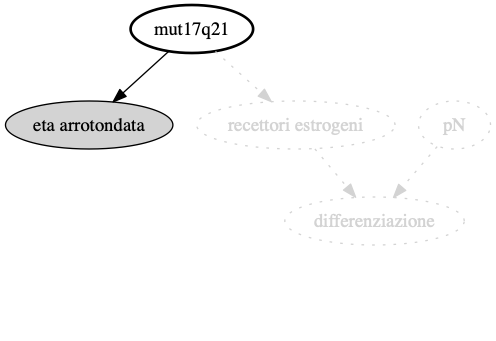
\includegraphics[width=0.5\textwidth]{mathematical-background/images/bn-example-separations-1}}
\caption{D-Separations in a subset of the provided data set (see Section \ref{sec:data-set})}
\label{fig:bn-separations-example-1}
\end{figure}

\begin{figure}[htbp]
\centerline{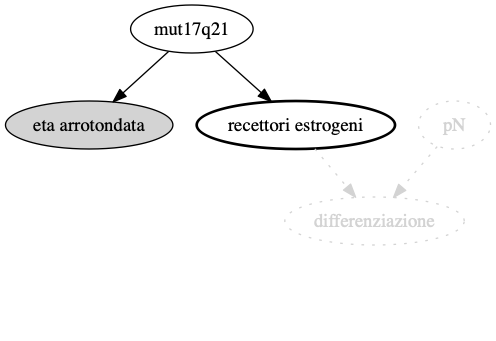
\includegraphics[width=0.5\textwidth]{mathematical-background/images/bn-example-separations-2}}
\caption{D-Separations in a subset of the provided data set (see Section \ref{sec:data-set})}
\label{fig:bn-separations-example-2}
\end{figure}

\begin{figure}[htbp]
\centerline{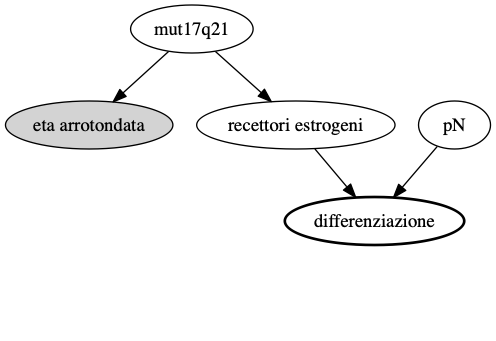
\includegraphics[width=0.5\textwidth]{mathematical-background/images/bn-example-separations-3}}
\caption{D-Separations in a subset of the provided data set (see Section \ref{sec:data-set})}
\label{fig:bn-separations-example-3}
\end{figure}
